\section{The TensorFlow Programming Model}\label{sec:model}

In this section we provide an in-depth discussion of the abstract computational
principles underlying the TensorFlow software library. We begin with an
examination of the basic structural and architectural decisions made by the
TensorFlow development team. Thereafter, we study TensorFlow's local as well as
distributed execution model. Lastly, we investigate how TensorFlow implements
back-propagation, a crucial step for many machine learning algorithms.

\subsection{Computational Graph Architecture}\label{sec:model-graphs}

In TensorFlow, machine learning algorithms are represented as
\emph{computational graphs}. A computational or \emph{dataflow} graph is a form
of directed graph where \emph{vertices} or \emph{nodes} describe operations,
while \emph{edges} represent data flowing between these operations. If an output
variable $z$ is the result of applying a binary operation to two inputs $x$ and
$y$, then we draw directed edges from $x$ and $y$ to an output node representing
$z$ and annotate the vertex with a label describing the performed
computation. Examples for computational graphs are given in Figure
\ref{fig:graphs}. The following paragraphs discuss the principle elements of
such a dataflow graph, namely \emph{operations}, \emph{tensors},
\emph{variables} and \emph{sessions}.

\begin{figure}
  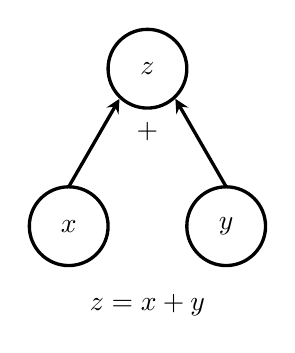
\begin{tikzpicture}
    % Result
    \draw [very thick] (1, 2) circle [radius=0.5cm] node {$z$};

    % Input Nodes
    \draw [very thick] (0, 0) circle [radius=0.5cm] node {$x$};
    \draw [very thick] (2, 0) circle [radius=0.5cm] node {$y$};

    % Edges
    \draw [very thick, -stealth] (0, 0.5) -- ++(60:1.29);
    \draw [very thick, -stealth] (2, 0.5) -- ++(120:1.29);

    % Operation Label
    \draw (1, 1.2) node {$+$};

    % Figure Label
    \draw (1, -1) node {$z = x + y$};
  \end{tikzpicture}
  %
  \hspace{0.2cm}
  %
  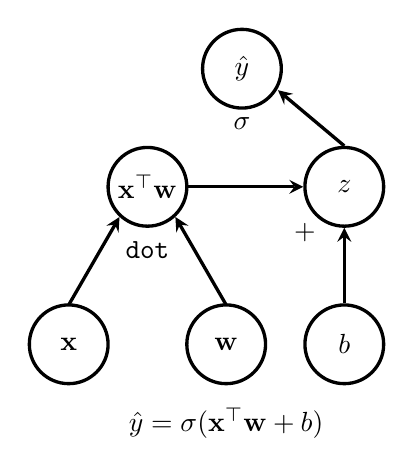
\begin{tikzpicture}
    % x^T w
    \draw [very thick] (1, 2) circle [radius=0.5cm] node {$\mathbf{x^\top w}$};

    % x and weights
    \draw [very thick] (0, 0) circle [radius=0.5cm] node {$\mathbf{x}$};
    \draw [very thick] (2, 0) circle [radius=0.5cm] node {$\mathbf{w}$};

    % Edges
    \draw [very thick, -stealth] (0, 0.5) -- ++(60:1.29);
    \draw [very thick, -stealth] (2, 0.5) -- ++(120:1.29);

    % Operation Label
    \draw (1, 1.2) node {\texttt{dot}};

    % Bias
    \draw [very thick] (3.5, 0) circle [radius=0.5cm] node {$b$};

    % z = (x^T w) + b
    \draw [very thick] (3.5, 2) circle [radius=0.5cm] node {$z$};

    % Operation label
    \draw (3, 1.42) node {$+$};

    % Edges
    \draw [very thick, -stealth] (3.5, 0.52) -- (3.5, 1.48);
    \draw [very thick, -stealth] (1.52, 2) -- (2.98, 2);

    % Sigmoid
    \draw [very thick] (2.2, 3.5) circle [radius=0.5] node {$\hat{y}$};

    % Operation label
    \draw (2.2, 2.8) node {$\sigma$};

    % Edge
    \draw [very thick, -stealth] (3.5, 2.52) -- ++(140:1.1cm);


    % Figure Label
    \draw (2, -1) node {$\hat{y} = \sigma(\mathbf{x}^\top \mathbf{w} + b)$};
  \end{tikzpicture}
  \caption{Examples of computational graphs. The left graph displays a very
    simple computation, consisting of just an addition of the two input
    variables $x$ and $y$. In this case, $z$ is the result of the operation $+$,
    as the annotation suggests. The right graph gives a more complex example of
    computing a logistic regression variable $\hat{y}$ in for some example
    vector $\mathbf{x}$, weight vector $\mathbf{w}$ as well as a scalar bias
    $b$. As shown in the graph, $\hat{y}$ is the result of the \emph{sigmoid} or
    \emph{logistic} function $\sigma$.}
  \label{fig:graphs}
\end{figure}

\subsubsection{Operations}\label{sec:model-graphs-ops}

The major benefit of representing an algorithm in form of a graph is not only
the intuitive (visual) expression of dependencies between units of a
computational model, but also the fact that the definition of a \emph{node}
within the graph can be kept very general. In TensorFlow, nodes represent
\emph{operations}, which in turn express the combination or transformation of
data flowing through the graph \cite{tensorflow}. An operation can have
\emph{zero or more} inputs and produce \emph{zero or more} outputs. As such, an
operation may represent a mathematical equation, a variable or constant, a
control flow directive, a file I/O operation or even a network communication
port. Table \ref{tab:ops} gives an overview of different kinds of operations
that may be declared in a TensorFlow graph.

\begin{table}[b!]
  \begin{tabular}{ll}
    \textbf{Category} & \textbf{Examples}
    \\ \toprule
    Element-wise operations & \texttt{Add}, \texttt{Mul}, \texttt{Exp}
    \\
    Matrix operations & \texttt{MatMul}, \texttt{MatrixInverse}
    \\
    Value-producing operations & \texttt{Constant}, \texttt{Variable}
    \\
    Neural network units & \texttt{SoftMax}, \texttt{ReLU}, \texttt{Conv2D}
    \\
    Checkpoint operations & \texttt{Save}, \texttt{Restore}
    \\ \bottomrule
    \end{tabular}
    \label{tab:ops}
    \caption{Examples for TensorFlow operations \cite{tensorflow}.}
\end{table}

Any operation must be backed by an associated implementation. In
\cite{tensorflow} such an implementation is referred to as the operation's
\emph{kernel}. A particular kernel is always specifically built for execution on
a certain kind of device, such as a CPU, GPU or other hardware unit.

\subsubsection{Tensors}\label{sec:model-graphs-tensors}

In TensorFlow, edges represent data flowing from one operation to another and
are referred to as \emph{tensors}. In the mathematical sense, a tensor is a
multi-dimensional collection of homogeneous values with a fixed, static type. In
terms of the computational graph, a tensor can be seen as a \emph{symbolic
  handle} to one of the outputs of an operation. A tensor itself does not hold
or store values in memory, but provides only an interface for retrieving the
value referenced by the tensor.

\subsubsection{Variables}\label{sec:model-graphs-vars}

Between two invocations of a computational graph, the majority of tensors in the
graph are destroyed and do not persist. However, it is often necessary to
maintain state across evaluations of a graph, such as for the weights and
parameters of a neural network. For this purpose, there exist \emph{variables}
in TensorFlow, which can be described as persistent, mutable handles to
in-memory buffers storing tensors. To manipulate and update variables,
TensorFlow provides the \texttt{assign} family of graph operations.

\subsubsection{Sessions}\label{sec:model-graphs-sessions}

In TensorFlow, the execution of operations and evaluation of tensors may only be
performed in a special environment referred to as \emph{session}. One of the
responsibilities of a session is to encapsulate the allocation and management of
resources such as variable buffers. Moreover, the \texttt{Session} interface of
the TensorFlow library provides a \texttt{run} routine, which is the primary
entry point for executing parts or the entirety of a computational graph. This
method takes as input the nodes in the graph whose tensors should be computed
and returned. Moreover, an optional mapping from arbitrary nodes in the graph to
respective replacement values --- referred to as \emph{feed nodes} --- may be
supplied to \texttt{run} as well \cite{tensorflow}. Upon invocation of
\texttt{run}, TensorFlow will start at the requested output nodes and work
backwards, examining the graph dependencies and computing the full transitive
closure of all nodes that must be executed. These nodes are then assigned to one
or many physical execution units (CPUs, GPUs etc.) on one or many machines.

\subsection{Execution Model}\label{sec:model-exec}

To execute computational graphs composed of the various elements just discussed,
TensorFlow divides the tasks for its implementation among four distinct groups:
the \emph{client}, the \emph{master}, a set of \emph{workers} and lastly a
number of \emph{devices}. When the client requests evaluation of a TensorFlow
graph via a \texttt{Session}'s \texttt{run} routine, this query is sent to the
master process, which in turn delegates the task to one or more worker processes
and coordinates their execution. Each worker is subsequently responsible for
overseeing one or more devices, which are the physical processing units for
which the kernels of an operation are implemented.

Within this model, there are two degrees of scalability. The first degree
pertains to scaling the number of machines on which a graph is executed. The
second degree refers to the fact that on each machine, there may then be more
than one device, such as, for example, five independent GPUs and/or three
CPUs. For this reason, there exist two ``versions'' of TensorFlow, one for local
execution on a single machine (but possibly many devices), and one supporting a
\emph{distributed} implementation across many machines and many devices. Figure
\ref{fig:exec} visualizes a possible distributed setup. While the initial
release of TensorFlow supported only single-machine execution, the distributed
version was open-sourced on April 13, 2016 \cite{tensorflowdist}.

\begin{figure}
  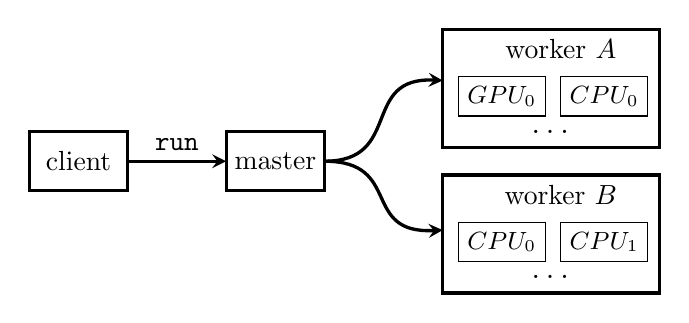
\begin{tikzpicture}
    % Client
    \draw [very thick] (0, 0) rectangle ++(1.25, 0.75) node [midway] {client};

    % Master
    \draw [very thick] (2.5, 0) rectangle ++(1.25, 0.75) node [midway] {master};
    \draw [very thick, -stealth] (1.25, 0.375) -- (2.5, 0.375) node [midway,
    above] {\texttt{run}};

    % Worker 1
    \draw [very thick] (5.25, 0.55) rectangle ++(2.75, 1.5);
    \draw (6.75, 1.8) node {worker $A$};
    \draw (5.45, 0.95) rectangle ++(1.1, 0.5) node [midway] {\small$GPU_0$};
    \draw (6.75, 0.95) rectangle ++(1.1, 0.5) node [midway] {\small$CPU_0$};
    \draw (6.65, 0.75) node {\large\dots};


    % Worker 2
    \draw [very thick] (5.25, -1.3) rectangle ++(2.75, 1.5);
    \draw (6.75, -0.05) node {worker $B$};
    \draw (5.45, -0.9) rectangle ++(1.1, 0.5) node [midway] {\small$CPU_0$};
    \draw (6.75, -0.9) rectangle ++(1.1, 0.5) node [midway] {\small$CPU_1$};
    \draw (6.65, -1.1) node {\large\dots};

    % Edges
    \draw [very thick, -stealth]
          (3.75, 0.375) .. controls +(1, 0) and (4.2, 1.45) .. (5.25, 1.4);
    \draw [very thick, -stealth]
          (3.75, 0.375) .. controls +(1, 0) and (4.2, -0.55) .. (5.25, -0.5);

  \end{tikzpicture}
  \caption{A visualization of the different execution agents in a multi-machine,
    multi-device hardware configuration.}
  \label{fig:exec}
\end{figure}

\subsubsection{Devices}\label{sec:model-exec-devices}

Devices are the smallest, most basic entities in the TensorFlow execution
model. All nodes in the graph, that is, the kernel of each operation, must
eventually be mapped to an available device to be executed. In practice, a
device will most often be either a CPU or a GPU. However, TensorFlow supports
registration of further kinds of physical execution units by the user. For
example, in May 2016, Google announced its \emph{Tensor Processing Unit} (TPU),
a custom built ASIC optimized specifically for fast tensor computations
\cite{tpu}. It is thus understandably easy to integrate new device classes as
novel hardware emerges.

\subsubsection{Placement Algorithm}\label{sec:model-exec-placement}

To determine what nodes to assign to which device, TensorFlow makes use of a
\emph{placement algorithm}. The placement algorithm simulates the execution of
the computational graph and traverses its nodes from input tensors to output
tensors. To decide on which of the available devices
$\mathbb{D} = \{d_1, \dots, d_n\}$ to place a given node $\nu$ encountered
during this traversal, the algorithm consults a \emph{cost model}
$C_\nu(d)$. This cost model takes into account four pieces of information to
determine the optimal device $\hat{d} = \argmin_{d \in \mathbb{D}} C_\nu(d)$ on
which to place the node during execution:

\begin{enumerate}
  \item Whether or not there exists an implementation (kernel) for a node on the
    given device at all. For example, if there is no GPU kernel for a particular
    operation, any GPU device would automatically incur an infinite cost.
  \item Estimates of the size (in bytes) for a node's input and output tensors.
  \item The expected execution time for the kernel on the device.
  \item A heuristic for the cost of cross-device (and possibly cross-machine)
    transmission of the input tensors to the operation, in the case that the
    input tensors have been placed on nodes different from the one currently
    under consideration.
\end{enumerate}

\subsubsection{Cross-Device Execution}\label{sec:model-exec-single}

If the hardware configuration of the user's system provides more than one
device, the placement algorithm will often distribute a graph's nodes among
these devices. This can be seen as partitioning the set of nodes into classes,
one per device. As a consequence, there may be cross-device dependencies between
nodes that must be handled via a number of additional steps. Let us consider for
this two devices $A$ and $B$ with particular focus on a node $\nu$ on device
$A$. If $\nu$'s output tensor forms the input to some other operations
$\alpha, \beta$ on device $B$, there conceptually exist cross-device edges
$\nu \rightarrow \alpha$ and $\nu \rightarrow \beta$ from device $A$ to device
$B$. This is visualized in Figure \ref{fig:cross-a}.

In practice, there must be some means of transmitting $\nu$'s output tensor from
$A$, say a GPU device, to $B$ --- maybe a CPU device. For this reason,
TensorFlow replaces the two edges $\nu \rightarrow \alpha$ and
$\nu \rightarrow \beta$ by two new nodes. On device $A$, a \texttt{send} node is
placed and connected to $\nu$. In tandem, on device $B$, a \texttt{recv} node is
instantiated and attached to $\alpha$ and $\beta$. The \texttt{send} and
\texttt{recv} nodes are then connected by an additional edge. This is shown in
Figure \ref{fig:cross-b}. During execution of the graph, cross-device
communication of data occurs exclusively via these special nodes.

\begin{figure}
  \centering
  %
  \begin{subfigure}[b]{0.30\textwidth}
    \centering
    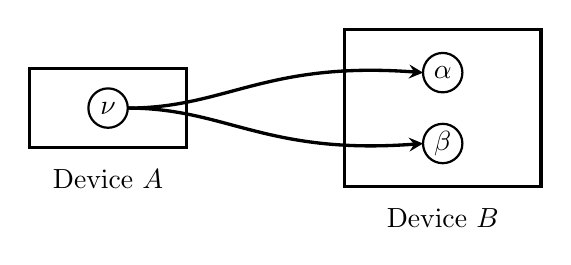
\begin{tikzpicture}
      % Device A
      \draw [very thick] (0, 0) rectangle (2, 1);
      \draw (1, -0.4) node {Device $A$};
      \draw [thick] (1, 0.5) circle [radius=0.25] node {$\nu$};

      % Device B
      \draw [very thick] (4, -0.5) rectangle (6.5, 1.5);
      \draw (5.25, -0.9) node {Device $B$};
      \draw [thick] (5.25, 0.05) circle [radius=0.25] node {$\beta$};
      \draw [thick] (5.25, 0.95) circle [radius=0.25] node {$\alpha$};

      % Edges
      % nu -> beta
      \draw [very thick, -stealth] (1.25, 0.5)
            .. controls (2.5, 0.5) and (3, 1.1)
            ..         (5, 0.95);
      % nu -> alpha
      \draw [very thick, -stealth] (1.25, 0.5)
            .. controls (2.5, 0.5) and (3, -0.1)
            ..          (5, 0.05);
    \end{tikzpicture}
    \caption{}
    \label{fig:cross-a}
  \end{subfigure}
  %
  \begin{subfigure}[h]{0.30\textwidth}
    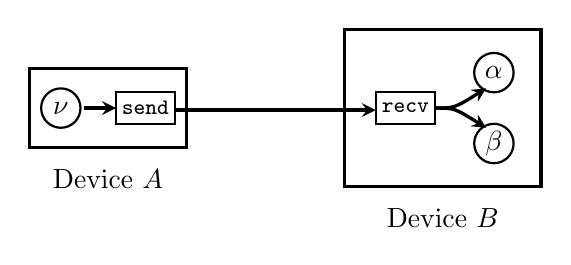
\begin{tikzpicture}
            % Device A
      \draw [very thick] (0, 0) rectangle (2, 1);
      \draw (1, -0.4) node {Device $A$};
      \draw [thick] (0.4, 0.5) circle [radius=0.25] node {$\nu$};

      % Device B
      \draw [very thick] (4, -0.5) rectangle (6.5, 1.5);
      \draw (5.25, -0.9) node {Device $B$};
      \draw [thick] (5.9, 0.05) circle [radius=0.25] node {$\beta$};
      \draw [thick] (5.9, 0.95) circle [radius=0.25] node {$\alpha$};

      % Send Nodes
      \draw [thick] (1.1, 0.3) rectangle ++(0.75, 0.4) node [midway]
      {\footnotesize\texttt{send}};
      \draw [very thick, -stealth] (0.7, 0.5) -- (1.1, 0.5);

      % Receive Nodes
      \draw [thick] (4.4, 0.3) rectangle ++(0.75, 0.4) node [midway]
      {\footnotesize\texttt{recv}};
      \draw [very thick, -stealth] (5.15, 0.5)
                      .. controls +(0.25, 0)
                               .. +(0.65, 0.25);
      \draw [very thick, -stealth] (5.15, 0.5)
                      .. controls +(0.25, 0)
                               .. +(0.65, -0.25);

      % Edges
      \draw [very thick, -stealth] (1.85, 0.475) -- (4.4, 0.475);
    \end{tikzpicture}
    \caption{}
    \label{fig:cross-b}
  \end{subfigure}
  \caption{A conceptual and practical visualization of cross-device
    communication. Figure \ref{fig:cross-a} shows the conceptual connections
    between nodes on different devices. Figure \ref{fig:cross-b} gives a more
    practical overview of how data is actually transmitted across devices using
    \texttt{send} and \texttt{recv} nodes.}
  \label{fig:cross}
\end{figure}

\subsection{Back-Propagation in TensorFlow}\label{sec:model-ext-backprop}

In a large number of deep learning and other machine learning algorithms, it is
necessary to compute the gradients of particular nodes of the computational
graph with respect to one or many other nodes. This is most often done via the
\emph{back-propagation} algorithm, which implements the chain rule. In
\cite{goodfellow2016}, two approaches for back-propagating gradients through a
computational graph are described. The first, which the authors refer to as
\emph{symbol-to-number differentiation}, receives a set of input values and then
computes the \emph{numerical values} of the gradients at those input values. It
does so by explicitly traversing the graph first in the forward order
(forward-propagation) to compute the cost, then in reverse order
(back-propagation) to compute the gradients. Another approach, more relevant to
TensorFlow, is what \cite{goodfellow2016} calls \emph{symbol-to-symbol
  derivatives} and \cite{tensorflow} terms \emph{automatic gradient
  computation}. In this case, gradients are not computed by an explicit
implementation of the back-propagation algorithm. Rather, special nodes are
added to the computational graph that calculate the gradient of each operation
and thus ultimately the chain rule. To perform back-propagation, these nodes
must then simply be executed like any other nodes by the graph evaluation
engine. As such, this approach does not produce the desired derivatives as a
numeric value, but only as a \emph{symbolic handle} to compute those values.

When TensorFlow needs to compute the gradient of a particular node $\nu$ with
respect to some other tensor $\alpha$, it traverses the graph in reverse order
from $\nu$ to $\alpha$. Each operation $o$ encountered during this traversal
represents a function depending on $\alpha$ and is one of the ``links'' in the
chain $(\nu \,\circ\, \dots\, \circ\, o \,\circ\, \dots)(\alpha)$ producing the
output tensor of the graph. Therefore, TensorFlow adds a \emph{gradient node}
for each such operation $o$ that takes the gradient of the previous ``link'' and
multiplies it with its own gradient. At the end of the traversal, there will be
a node providing a symbolic handle to the overall target derivative
$\frac{d\nu}{d\alpha}$, which \emph{implicitly} implements the back-propagation
algorithm. Figure \ref{fig:gradients} shows how a computational graph may look
before and after gradient nodes are added.

\begin{figure}
  \centering
  \begin{subfigure}[b]{0.2\textwidth}
    \centering
    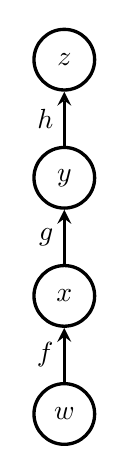
\begin{tikzpicture}
      % Nodes
      \path [very thick] (0, 0)
            coordinate [draw, circle, text width=0.5cm] (w) node {$w$};
      \path [very thick] (0, 1.5)
             coordinate [draw, circle, text width=0.5cm] (x) node {$x$};
      \path [very thick] (0, 3)
            coordinate [draw, circle, text width=0.5cm] (y) node {$y$};
      \path [very thick] (0, 4.5)
            coordinate [draw, circle, text width=0.5cm] (z) node {$z$};

      % Edges
      \draw [very thick, -stealth] (w) -- (x) node [midway, left] {$f$};
      \draw [very thick, -stealth] (x) -- (y) node [midway, left] {$g$};
      \draw [very thick, -stealth] (y) -- (z) node [midway, left] {$h$};
    \end{tikzpicture}
    \caption{}
    \label{fig:gradients-a}
  \end{subfigure}
  \begin{subfigure}[b]{0.2\textwidth}
    \centering
    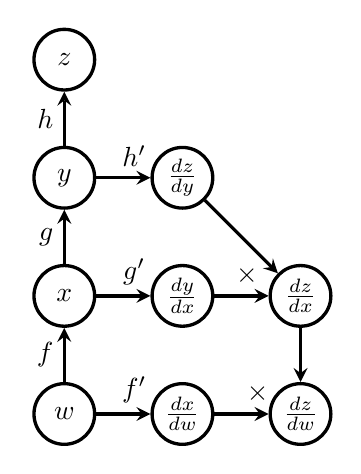
\begin{tikzpicture}
      % Nodes
      \path [very thick] (0, 0)
            coordinate [draw, circle, text width=0.5cm] (w) node {$w$};
      \path [very thick] (0, 1.5)
             coordinate [draw, circle, text width=0.5cm] (x) node {$x$};
      \path [very thick] (0, 3)
            coordinate [draw, circle, text width=0.5cm] (y) node {$y$};
      \path [very thick] (0, 4.5)
            coordinate [draw, circle, text width=0.5cm] (z) node {$z$};

      % Edges
      \draw [very thick, -stealth] (w) -- (x) node [midway, left] {$f$};
      \draw [very thick, -stealth] (x) -- (y) node [midway, left] {$g$};
      \draw [very thick, -stealth] (y) -- (z) node [midway, left] {$h$};

      % Derivatives
      \path [very thick] (1.5, 0)
            coordinate [draw, circle, text width=0.5cm] (wp) node {$\frac{dx}{dw}$};
      \path [very thick] (1.5, 1.5)
             coordinate [draw, circle, text width=0.5cm] (xp) node {$\frac{dy}{dx}$};
      \path [very thick] (1.5, 3)
            coordinate [draw, circle, text width=0.5cm] (yp) node {$\frac{dz}{dy}$};

      % Edges
      \draw [very thick, -stealth] (w) -- (wp) node [pos=0.7, above] {$f'$};
      \draw [very thick, -stealth] (x) -- (xp) node [pos=0.7, above] {$g'$};
      \draw [very thick, -stealth] (y) -- (yp) node [pos=0.7, above] {$h'$};

     % Chain Rule
      \path [very thick] (3, 0)
            coordinate [draw, circle, text width=0.5cm]
            (dzdw) node {$\frac{dz}{dw}$};
      \path [very thick] (3, 1.5)
             coordinate [draw, circle, text width=0.5cm]
             (dzdx) node {$\frac{dz}{dx}$};

      % Edges
      \draw [very thick, -stealth] (wp) -- (dzdw)
            node [pos=0.8, above] {$\times$};
      \draw [very thick, -stealth] (xp) -- (dzdx)
            node [pos=0.6, above] {$\times$};
      \draw [very thick, -stealth] (yp) -- (dzdx);
      \draw [very thick, -stealth] (dzdx) -- (dzdw);
    \end{tikzpicture}
    \caption{}
    \label{fig:gradients-b}
  \end{subfigure}
  \caption{A computational graph before (\ref{fig:gradients-a}) and after
    (\ref{fig:gradients-b}) gradient nodes are added. In this
    \emph{symbol-to-symbol} approach, the gradient $\frac{dz}{dw}$ is just
    simply an operation like any other and therefore requires no special
    handling by the graph evaluation engine.}
  \label{fig:gradients}
\end{figure}

%%% Local Variables:
%%% mode: latex
%%% TeX-master: "../paper"
%%% End: